\chapter{Implementation}

\underline{\textbf{\LARGE //TODO:}} skriv om.
The main part of implementing the parser was to rewrite the EBNF provided by W3C in \cite{w3c01} to conform to ANTLR's syntax and semantics. In the following chapter we will present the reason why this was not a trivial task, the ambiguous terminals, and by which means we solved this. In addition we will present other ANTLR conforformity rewrites and finally our implementation of scoping and symbol tables.

\underline{\textbf{\LARGE //ODOT:}}

\section{ANTLR Syntax Conformity}
The W3C(\cite{w3c00}) and ANTLR(section \ref{sect:antlr:grammarSpec}) EBNF syntax differs in multiple ways. Some of the differences are trivial, e.g. the "defined by"-operator, which in W3C syntax is denoted with \verb!::=! and in ANTLR syntax as \verb!:!. Such differences can be fixed by means of a simple symbol replacement. However, the W3C metagrammar also embodies some operators such as the 'hat' and the 'dash' operators, described in section \ref{sect:ambiguousgrammar:ambigTerm}, of which there are no complete equivalents in the ANTLR metagrammar. In addition, the W3C grammar defines some producions as terminal and other as non-terminal, but this division does not hold for all implementations.

\subsection{Seperating Parser and Lexer Rules}

The ANTLR parser generator can generate parsers and lexers from a single grammar file. The distinction between terminals and non-terminals is that terminals start with \emph{uppercase} letters, and non-terminals start with \emph{lowercase} letters. Which productions to go where is highly dependant on what strategy we chose to solve the ambigious terminals problem. E.g. by defining all the ambigious terminals as non-terminals we would have solution very close to a scan-while-parse scanner (section \ref{sect:ambiguousgrammar:scanWhileParse}). Because we chose the strategy of letting the parser control the lexer's state, we could define a division of terminals and non-terminals very similar to the one specified by W3C. The exception is \verb!QName!, which by W3C is defined as follows:
\begin{verbatim}
QName           ::= PrefixedName
                  | UnprefixedName
PrefixedName    ::= Prefix ':' LocalPart 
UnprefixedName  ::= LocalPart 
Prefix          ::= NCName
LocalPart       ::= NCName
\end{verbatim}
Where \verb!NCName! is another terminal, thus creating an easily solvable ambiguity. It is possible to rank the \verb!QName! production higher than the \verb!NCName! with a syntactic predicate checking if the token after \verb!NCName! is a \verb!':'!, but there is no good reason for doing so, when it can be defined as a non-terminal in this way:
\begin{verbatim}
qName             : (NCName COLONSi)? NCName;
\end{verbatim}
There is however a reason for \emph{not} defining \verb!QName! as a terminal: by doing so, ANTLR would have generated token containing the whole \verb!QName!, meaning that e.g. if one is only interested in the localpart, one would have to manually split the text.

\subsection{Rewriting the W3C 'dash' and 'hat' operators}
The 'hat' operator (section \ref{sect:ambiguousgrammar:ambigTerm}) is mostly used to define legal characters by defining which are illigal. These productions can be rewritten in ANTLR syntax by using the not-operator ($\sim$) and a \verb!fragment! production rule \verb!NotChar! which is manually defined as all unicode characters (up to 0xFFFF, see section \ref{sect:parserconstructanddebug:limitations}) not allowed by the W3C defined \verb!Char!:
\begin{verbatim}
// The extracted part of StringLiteral:
PartOf          ::= [^"&]

// can be written in ANTLR syntax as:
PartOf            : ~(NotChar | COLONSi | AMPSi);
\end{verbatim}
The 'dash' operator is sometimes also used like this, like in e.g. \verb!QuotAttrContentChar! but because of our introduced production \verb!QuotAttributeContent! (section \ref{sect:rewriteGrammar:reorganizing}) it is rewritten in the same way as with the enclosed expressions (section \ref{sect:rewriteGrammar:enclosedComposite}), where the operator is used to define that a very gereral production should not be greedy. 

In \verb!piTarget! the 'dash' operator is used in a unique way, and thus needed to be treated differently:
\begin{verbatim}
// Original production
PiTarget    ::= Name - (('X' | 'x') ('M' | 'm') ('L' | 'l'))

// Rewritten production using a semantic predicate
piTarget    : n=Name { !$n.getText().equalsIgnoreCase("XML") }?;
\end{verbatim}
Where the original production can be interpreted as ``piTarget can be a Name, but not `XML', regardless of character casing''. The validating semantic predicate will imitate this behaviour using the method \verb!equalsIgnoreCase()!.

\section{Parser Controlled State Driven Lexer}

\textbf{\LARGE //TODO:} 

Kjempetvetydigheten med ElementContentChar / AttributeContentChar / NCName etc. \\
Systemet med states, stack og parser snakker direkte til lexer

\textbf{\LARGE //TODO:} 

\subsection{UnbufferedCommenTokenStream}
\textbf{\LARGE //TODO:}  

Omskriving av TokenStream for at den ikke skal buffre mer en strengt tatt nodvendig

\subsection{Reorganizing the Grammar}
\label{sect:rewriteGrammar:reorganizing}
\textbf{\LARGE //TODO:} 

Slik at state-systemet fungerer: Lage fragment av alt, nye tokens (ElementContent), TOKENSWITCH, semantiske predikat, etc.

\subsection{State Transitions}
\textbf{\LARGE //TODO:} 

Hvordan parseren gaar over fra en state til en annen, systemet med stack.

\section{Enclosed Composite Lexer Productions}
\label{sect:rewriteGrammar:enclosedComposite}
\textbf{\LARGE //TODO:} 

Regler som PI, Pragma, XMLComment and CDATA kan fanges i sin helhet i lexeren. Samme med saertilfellet XQuerykommentarer. 

Fint for aa skille alternativer, men man ikke faar tak i deltokens... saa derfor ----v

\subsection{Emiting More Than One Token Per Production}
\textbf{\LARGE //TODO:} 

Omskriving av lexer for a la produksjoner avgi mer enn ett token

\subsection{PI, Pragma, XMLComment and CDATA Sections}
\textbf{\LARGE //TODO:} 

Sammensatte omhyllede lexerregler (<? noe ?>, <!-- noe --> etc)

\subsection{Nested XQuery Comments}
XQuery allows nested comments, for example:
\begin{verbatim}
(: this is a comment (: this comment is nested :) :)
\end{verbatim}
This is a classic problem in compiler construction, however it can be solved using standard ANTLR syntax, without resorting to custom functions/methods for consuming input and keeping track of nesting. The original EBNF as specified by W3C is as follows:
\begin{verbatim}
Comment ::= "(:" (CommentContents | Comment)* ":)"
\end{verbatim}
At first glance, this seems uncomplicated and straight forward, but this grammar needs to be rewritten to be accepted by an LL parser. A suggestion for a solution to this problem was initially found on the Antlr mailing list\footnote{http://www.antlr.org:8080/pipermail/antlr-interest/2005-July/012967.html}, and we loosly based our implementation on such an approach. This lexer rule will correctly detect and allow nested comments, and hide them from the parser:
\begin{verbatim}	
Comment   : LXQCOMMENTSi 
           ({(input.LA(1)=='(' && input.LA(2)==':')}?Comment 
           | {input.LA(2)!=')'}?=>COLONSi
           | {input.LA(2)!=':'}?=>LPARSi
           | ~(LPARSi | COLONSi | NotChar))*
            RXQCOMMENTSi; {$channel=HIDDEN;}
    fragment LXQCOMMENTSi     : '(:';
    fragment RXQCOMMENTSi     : ':)';
\end{verbatim}
Where the disambiguating semantic predicate on the second line can be understood as "if it looks like a comment, it is a comment". The gated semantic predicates on the third and fourth line guards the production from being greedy, i.e. they hide the posibility of matching a \verb!':'! if it is followed by a \verb!')'!, and \verb!'('! if it is followed by a \verb!':'!. By using \verb!$channel=HIDDEN! ANTLR will put this token in an different virtual channel than the default one, making it invisible for the parser unless explicitly asked for. 

\section{Differentiating NCName and Keywords}

\textbf{\LARGE //TODO:} 

Systemet med NCNames vs keywords. \\
Husk: Keywords er uttrykt som tokens for aa sperre av for parsing og for oversiktlige feilmeldinger.

\section{Extra-grammatical Constraints}

\textbf{\LARGE //TODO:} 

Whitespace, leading dash etc..

\section{Resolving Non-determinisms in the Parser }

\textbf{\LARGE //TODO:} 

pathExpr og itemtype occurenceindicator trengte syntaktiske predikat

\section{Reserved Keywords}

\underline{\textbf{\LARGE //TODO:}} dette maa flyttes eller skrives om.

A particular feature in XQuery is the lack of reserved keywords. This creates a
series of problems when a lexer based on the verbatim grammar specification from
the W3C is trying to recognize tokens. 

vaar parser har enna reserved keywords, flytte dette til future work? \\
\underline{\textbf{\LARGE //ODOT:}} 




% Discussion / ScopingAndSymbol
\section{Scoping, Symbol Tables, and Typechecking}
In this section we will discuss scoping, symbol tables, and type
checking/inference.

\subsection{Scoping and Symbol Tables on AST}
Currently the scoping and symbol tables are being used directly in the grammar -
that is, during parse time, as described in section
\ref{sect:impl:scoping_and_symtab}. It would be benefitial to move this
functionality into being performed in run time, and combine with type checking
functionality. This possibility was previously mentioned in section
\ref{sect:discussion:ast:extend}.

This would decouple some amount of code from the grammar, improving readability
slightly and creating more self-contained parser with no forced semantic checks
since this would be implemented in the AST parser instead.

The current implementation is adequate, but maintainability and extendability
suffers from the constraints of being locked into a monolithic grammar file.

\subsection{Type Checking}
Currently the parser will not perform type checking on the parsed queries. This
is an essential feature and will be necessary to implement for the parser to be
applicable in any realistic setting. A type checking system with proper type
inference and synthesis could be a complex feature to implement in a language
such as XQuery, and might require considerable effort, especially in quality
assurance. 

However, the resulting AST output from the parser (presented in section
\ref{sect:results:parser_output_ast}) should be a solid base to improve upon by
adding proper type inference and type checking. This would require a framework
for dataflow analysis. This is a substantial amount of work, but it would
benefit the project in several ways, for example the possibility of adding
optimizations.
% Implementation: error handling
\section{Error Handling}
\label{sec:impl:errorhandling}
\begin{figure}[!h]
  \centering
    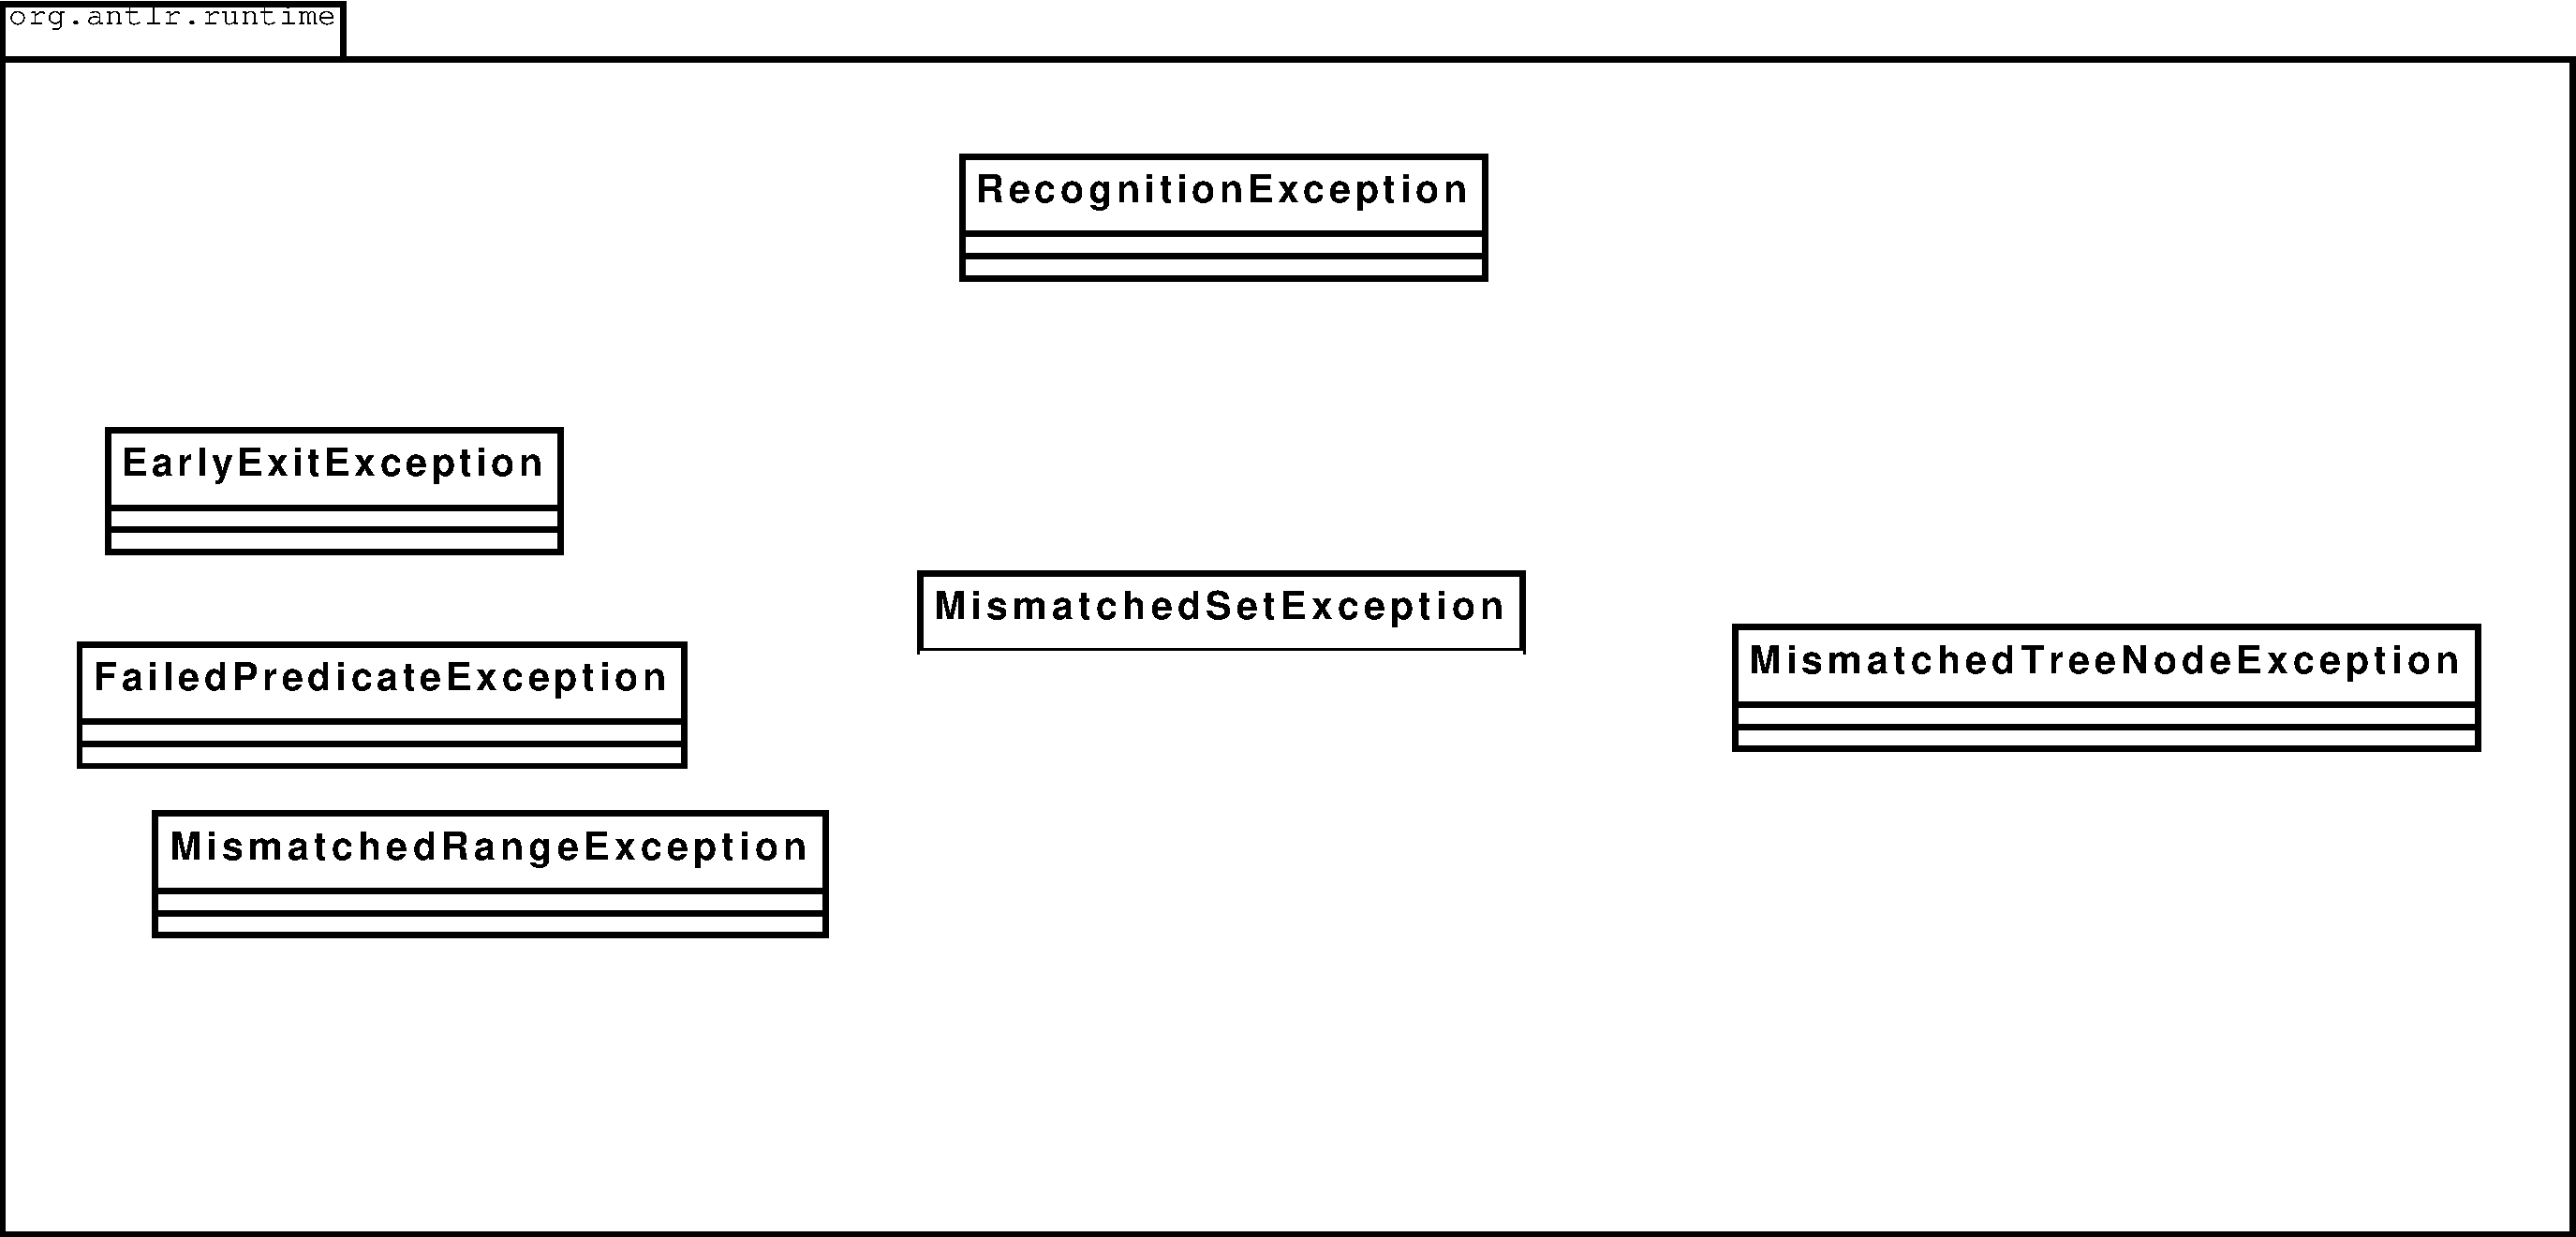
\includegraphics[width=1\textwidth]{diagrams/exception_uml}
  \caption{ANTLR exceptions class hierarchy}
\label{fig:antlrException}
\end{figure}
Error handling in ANTLR is initially done by catching exceptions and printing
an error message to stderr. The parser will then attempt to recover from the
error and continue parsing. This behaviour is not always desirable, so certain
methods were overridden to allow exceptions to be thrown upwards the stack to
the program that initiated the parser (the calling program, or top-level
program). An overview of the posible exceptions ANTLR can throw is shown in figure \ref{fig:antlrException}.

Specifically, this was done by overriding the methods \verb!mismatch()! as well as
\verb!recoverFromMismatchedSet()!, as such:

\begin{Verbatim}
    protected void mismatch(IntStream input, 
                            int ttype, 
                            BitSet follow)
        throws RecognitionException
    {
        throw new MismatchedTokenException(ttype, input);
    }

    public void recoverFromMismatchedSet(IntStream input, 
                                         RecognitionException e, 
                                         BitSet follow)
        throws RecognitionException
    {
        throw e;
    }
\end{Verbatim}

Additionally, a special \verb!@rulecatch! rule had to be added to force ANTLR from
handling errors and instead throwing the exceptions upwards:

\begin{Verbatim}
@rulecatch {
    catch (RecognitionException e) {
        throw e;
    }
}
\end{Verbatim}

However, some exceptions thrown by the lexer were impossible to handle - these
were handled in the \verb!nextToken()! method in the \verb!Lexer! superclass.
This issue has been documented in section 
\ref{sect:error_handling:syntax_errors}.

